\chapter{Introduction}
\lhead{Chapter 1 \emph{Introduction}}
\label{chap:1}
%\autoref{chap:1}

\section{Motivation}
\bigskip
\bigskip

In 1957 the first satellite in history was launched and since then thousands other objects were placed into orbit. \cite{Belward 2015}, \cite{ESA 2019} Two decades later NASA’s scientist Kessler proposed a scenario, in which he theorized that the increasing density of the objects in the Low Earth Orbit (LEO) cause collisions and the generated space debris increase even more the probability of further collisions. The humanity today is confronted more than ever with the realization of this theory, which has gone down as Kessler Syndrome.

There have been taken many important steps towards raising the consciousness about the overpopulation problem, as well as the enactment of rules regarding the capacity and orbit allocation. However, despite the fact that coordination committees and working groups have been established and they are involved in the mitigation guidelines, the existed space traffic management rules deals today only with the frequency allocation used by satellites.

Having said that, the motivation of this thesis is the creation of an application, which will help into supplementing the space traffic management rules regarding the physical location of satellites based on the added value that each satellite contributes to the society in terms of additional services or data. This application is focused on Earth Observation (EO) satellites at LEO, which is one attempt to approach and tackle the problem. In conjunction with a database, which hosts information about the EO satellites that are currently on orbit at LEO, the application also offers the following service. The user can find out about the existing orbiting and operational EO satellites or constellations that provide the outcome/ service that he/she asked for.

\bigskip
\bigskip

\newpage
\section{Scope and key assumptions}
\bigskip

%\textit{Edit it...}

The first part of this work pertains to the Theoretical Framework of the discussed problem; the overpopulation. The points being addressed are: the problem of overpopulation, the concept of orbital capacity, the state of LEO and its critical regions, the basic characteristics of LEO, the different ways of dealing with the problem, as well as the mitigation guidelines, which have been already put into action.

The second part of this master thesis is dedicated to the development of an application, which can give the incentives to create space traffic management rules based on the orbit and capacity allocation, as well as the added value that each new satellite provides. More specifically, the concept of added value is based on the idea that each new satellite is prioritized to be launched when it provides some additional services or data to the society, which are not offered from another existing and functional satellite/ constellation.
%It is not monetary.

One attempt to approach the development of such application is to focus on Earth Observation (EO) satellites at LEO. The reason behind the selection of EO as the first group of satellites to be tested in the application, is because the calculation and evaluation of the capabilities of an EO satellite is more apparent in comparison to other scientific or technological missions. This also applies to the field of telecommunication, in which there is a competition between the satellite and terrestrial industry and thus the estimation of the added value that each satellite provides to the society is more complex to be defined. Ultimately, this application focus on EO satellites in LEO and has 3 capabilities.
%

\begin{itemize}
\item The first capability is that the user can define a satellite mission or constellation, which means that the number of satellites, the altitude, the orbital plane, resolution etc. is known. Then, the software can answer what is the revisit time of that defined mission in a certain area.
\item The second capability is the following: The actual outcome/service of a Earth Observation satellite is defined. Namely, if such is images from the visual band of entire Earth, which have a certain revisit time and resolution, then the software can provide to the user the orbital characteristics of the satellite or constellation that can supply the desired data.
\end{itemize}

An extension of this application and its capabilities is the creation of a small database of Earth Observation satellites.

\begin{itemize}
\item In both mentioned capabilities of the application, the user can find out, if there are currently satellites which offer the desired data that they had asked for and if such satellites exist, to name them.
\end{itemize}

The database contributes greatly to the creation of a well-rounded application, which can help into mitigating the problem of overpopulation. Since the user can find out which satellites do a certain/asked project or if they offer a specific service, thus he/she can decide whether a new satellite is needed to be launched based on whether the desired service is offered or not by someone else. In this way, it can also incentivize in the future companies to cooperate with each other, instead of constructing/ designing/ launching a new constellation. Thus, a rule in the field of space traffic management can be formulated based on the added value that a new satellite offers.

%Lastly, the part of the Evaluation follows, as well as parts of Summary and Conclusions and that of Future work.

%Space sustainability!


\section{Current launching trend}
\bigskip

%Current launching trend

Having said that, the current trend is that the world goes in the direction of launching more and more small satellites, which are most of the times parts of large constellations aiming at providing persistent global internet. The reason that lies behind is that the commercial space industry has benefits such low costs and increased competition. Nevertheless, the notion of proliferated constellations is propitiatory for the future. This is because it provides more resilience, since the loss of a satellite will not hamstring the whole constellation and the mission can continue.

(especially in LEO)
(Fig. \ref{launch_traffic_LEO}) (Fig. \ref{launch_traffic_GEO}) 

\begin{figure}
\centering
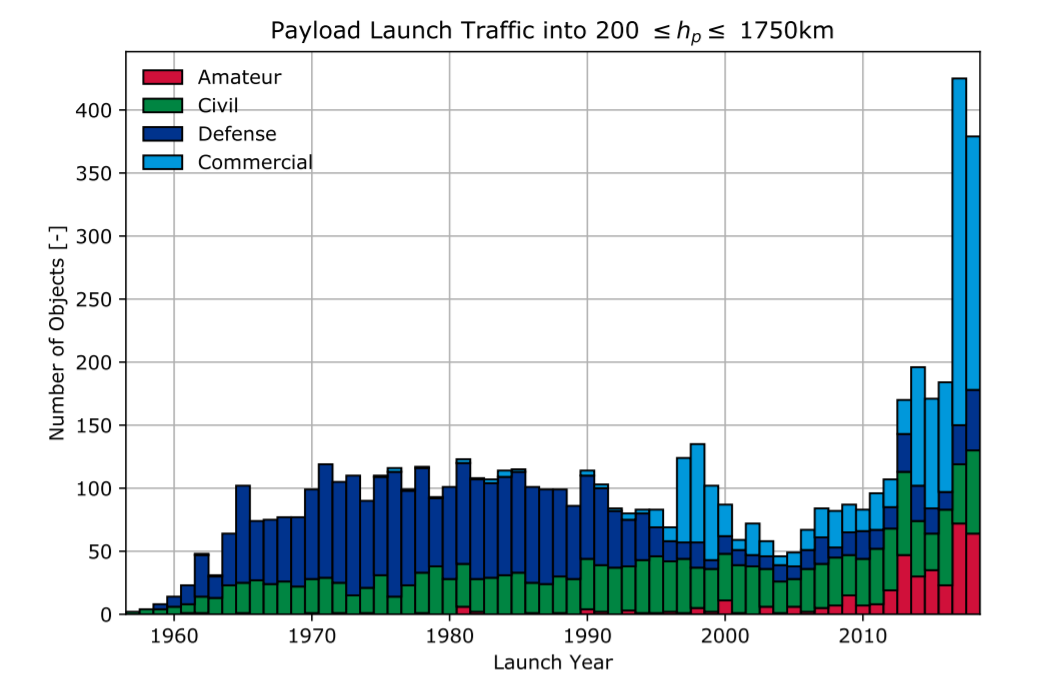
\includegraphics[width=0.9\textwidth]{Images/launch_traffic_LEO.png}\caption{Payload launch traffic into LEO (1957-2019). \textit{Source: \cite{ESA 2019}}}
\label{launch_traffic} 
\end{figure}

\begin{figure}
\centering
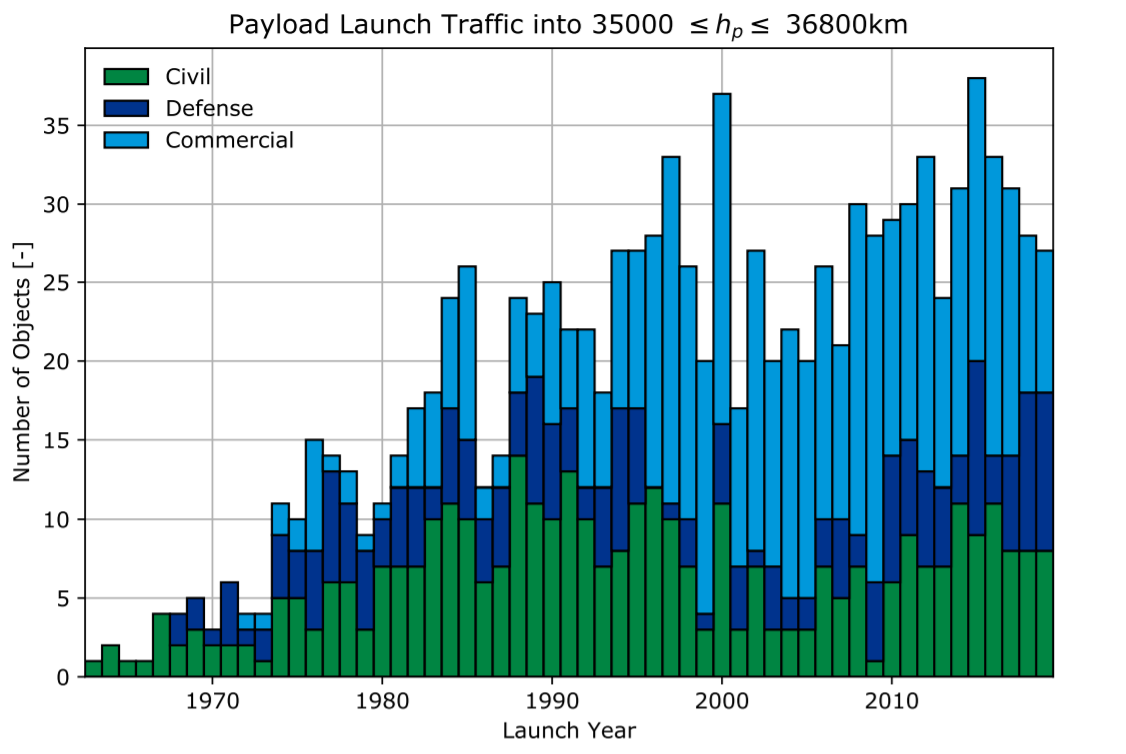
\includegraphics[width=0.9\textwidth]{Images/launch_traffic_GEO.png}\caption{Payload launch traffic into GEO (1957-2019). \textit{Source: \cite{ESA 2019}}}
\label{launch_traffic} 
\end{figure}



It seems that space nowadays can be linked to the phenomenon of Tragedy of Commons. Based on this concept written by the British economist Lloyd, the shared-resource system is spoiled by individual users who act based on their own benefit and against the common good. This notion describes the current situation of the space industry. +++ non-infinite environment +++ At the same time the "no ownership in space" gave the permission to people....

%the current situation of the big constellations (e.g. Starlink)